\section{Part 2: Invasive Species Trade-Off Model}

\subsection{Problem Analysis}
As with most events, the growth of foreign plants comes with benefits and drawbacks. Thus, to develop an invasive species impact score, we divide the impact into two primary categories: ecological impact and economic potential (see Figure~\ref{fig:invasiveimpactbrainstorm}). Through this concept, we can represent our "impact factor" as the trade-off between ecological and economic impacts. 

\begin{figure}[h!]
\centering
    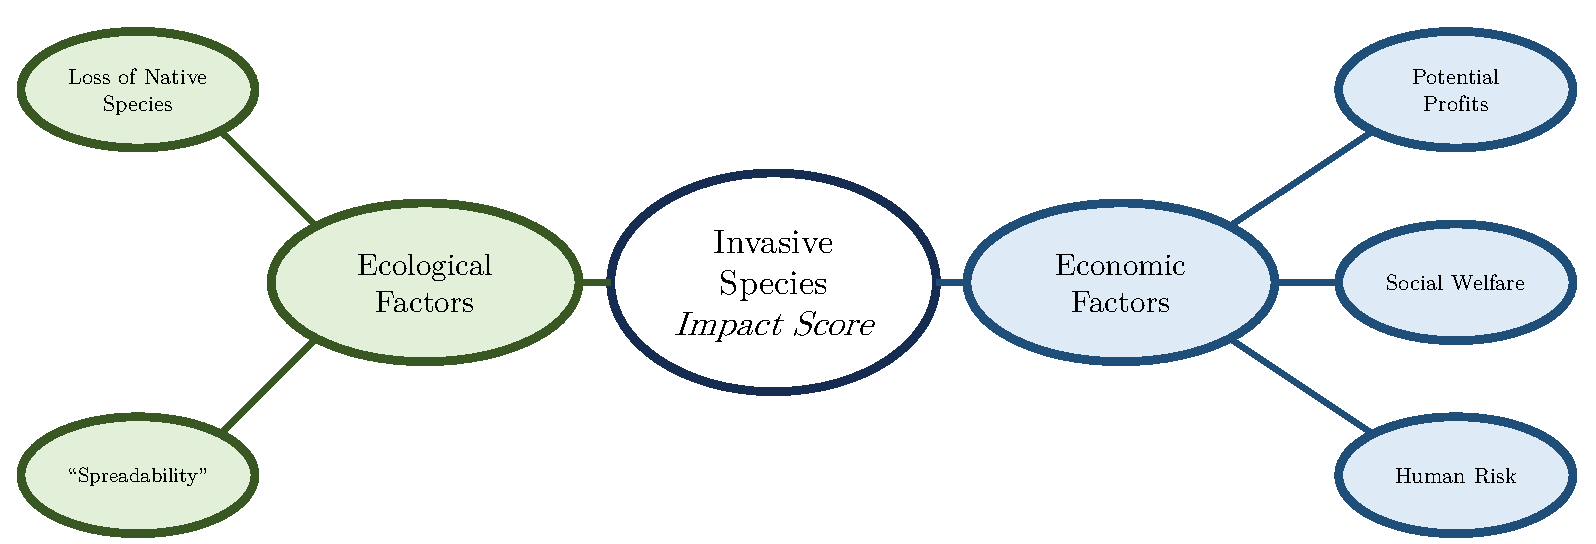
\includegraphics[scale=0.5]{figures/invasivespeciesimpactscore.pdf}
    \captionsetup{width=0.9\textwidth}
    \caption{\textbf{Overview of trade-off model.}}
    \label{fig:invasiveimpactbrainstorm}
\end{figure}

\subsection{Model Overview}

Invasive species are non-native organisms that typically out-compete native species because of their ability to reproduce aggressively. Invasive species often harm their surrounding environments by disrupting food chains, which further causes ecological imbalance. 

In the following section, we define \textit{foreign species} as a non-native species introduced to a new region of interest. Furthermore, we define \textit{spreadability} as the ease with which a foreign species can proliferate on a rural plot of land. We believe our proposed trade-off model will determine a species as invasive or simply foreign. Our model is useful for all perspectives because we model the "impact factor" as a comparison between the risks and rewards associated with foreign plants in a new environment. 



\subsection {Assumptions \& Variables}

In addition to our assumptions from Part 1, we provide more assumptions specific to Part 2 below. The following list of variables summarizes the key components of our trade-off model. We will derive each of the following functions (or scores) in this section.

\begin{table}[h!]
\renewcommand{\arraystretch}{1.3}
    \begin{tabularx}{\textwidth}{lp{0.4\textwidth}X}
    \toprule
    \textbf{\#} & \textbf{Assumption} & {\centering \textbf{Justification}}  \\ \midrule
    
    \raggedright \nextassumption\label{assumption:10} & Native species are in competitive equilibrium before introducing a foreign species. & This key assumption allows us to use the Lotka-Volterra equations to compare before and after effects.\\
    
    \rowcolor{gray!15} \raggedright \nextassumption\label{assumption:11} & Foreign species populations grow logistically with a set carrying capacity. & This allows us to create a standardized metric based on logistic regression for measuring population growth.
 \\

 \raggedright \nextassumption\label{assumption:12} & A foreign species' social benefit and human health risk can be measured in dollars. & Measuring societal impacts in dollars allows us to create another standardized measure. \\
 
    \bottomrule
    \end{tabularx}
\end{table}

\begin{table}[h]
\renewcommand{\arraystretch}{1.3}
%p{0.8\linewidth
    \begin{tabularx}{\textwidth}{p{0.2\textwidth}lX}
    \toprule
    \textbf{Variable}           & \textbf{Symbol} & \textbf{Description}  \\ \midrule
    \raggedright Native Species Population Changes & $\chi$  & Sum of changes in native species' population after introducing a foreign species (measured as a proportion). \\
    \rowcolor{gray!15}
    \raggedright Spreadability Rate  & $r$  & Rate of uninterrupted logistic growth of foreign species.\\
    Economic Profit & $\pi$  & Potential profit (USD) from a business centered around a foreign species. \\
    \rowcolor{gray!15} \raggedright Social Welfare Benefit& $W$   & Implicit social benefit (measured in USD) from a foreign species. \\
    \raggedright Human Health Risk & $R$ & Potential risk (measured in USD) of a foreign species to humans.\\
    \bottomrule
    \end{tabularx}
\end{table}

\subsection{Ecological Impact Score}

To begin, we determine two main measures of a foreign species' ecological impact: the overall change in the population of the native species and the rate at which a foreign species can spread (spreadability). Therefore, we formulate an ecological impact score as a combination of these factors, none of which are dispositive. 

\subsubsection{Effects on Native Species}

To analyze the impacts of a foreign species in a new region, we need to measure the unintended consequences on native populations. To do so, we used the Lotka-Volterra model (a system of differential equations) to represent the changes in each native population. The Lotka-Volterra model is commonly used to analyze competing species' population dynamics, especially in our case between foreign and native species \cite{noauthor_lotka-volterra_nodate}. 

Assuming native species are in competitive equilibrium before the introduction of a new, foreign species (Assumption~\ref{assumption:10}), we can use a generalized system of Lotka-Volterra equations for \(n\) native species, where we can treat population growth for each species as a single vector based on the populations of other species at each time step. Additionally, we use a matrix to model the weightings of how other native populations affect the growth of another species.

Mathematically, we let there be \(n\) native species where the population of a native species \(i\) where \(1 \leq i \leq n\) is denoted by \(x_i\). Therefore, the rate of change of a population \textit{in relation to} other species can be represented as 

\begin{equation}
    \frac{dx_i}{dt} = r_ix_i \left(1 - \frac{\sum\limits_{j=1}^n \alpha_{ij} x_j}{K_i}\right)
    \label{eq:lotkavolterra}
\end{equation}

where \(r_i\) is the uninterrupted growth rate of species \(i\), \(\alpha_{ij}\) is the impact of species \(j\) on species \(i\), and \(K_i\) is the carrying capacity of species \(i\). The parameters \(\alpha_{ij}\) can be combined into an \(n\) by \(n\) matrix of "interaction" parameters. Therefore, we denote this matrix of parameters the \textit{interaction matrix}. For the first \(n\) native species, the Lotka-Volterra equations will yield a system of \(n\) differential equations with an \(n\) by \(n\) matrix \(\alpha\). When we introduce our new foreign species, the Lotka-Volterra model will yield a system of \(n+1\) differential equations with an interaction matrix \(\alpha\) of dimensions \(n+1\) by \(n+1\) where all values \(\alpha_{ii} = 1\) for self-interaction of species. See Equation~\ref{eq:alphaexample} for an example interaction matrix of three native species and one foreign species.

\begin{equation}
        \alpha_{\text{ foreign species}} = {\underbrace{\begin{bNiceMatrix}[first-row,first-col]
        &&&&& \\
    \text{Native Species 1} && 1 & \alpha_{1,2} & \alpha_{1, 3} & \alpha_{1, 4} &\\
    \text{Native Species 2} && \alpha_{2, 1} & 1 & \cdots & \cdots &\\
    \text{Native Species 3} && \alpha_{3, 1} & \cdots & 1 & \cdots  &\\
    \text{Foreign Species} && \alpha_{4, 1} & \cdots & \cdots & 1 & \\
    \end{bNiceMatrix}}_{ \\ \text{3 native species, 1 foreign species.}}}
    \label{eq:alphaexample}
\end{equation}

We used SciPy, a scientific software, to obtain numerical solutions (\(x_i\)) to the Lotka-Volterra system \cite{scipy}. With population functions \(x_i\), we can model the populations over time. For simplicity's sake, we assume that the changes in populations of 3 native species are representative enough of the impact of each foreign species. To create a standardized score, we developed a native population impact score, which measures the change of a native species' population as a ratio after one year since introducing a new foreign species. We call the sum of these ratios our native species impact score, represented by \(\chi\).

\begin{equation}
    \chi = \sum_{i = 1}^n \frac{x_i {\text{ new}}}{x_i {\text{ old}}}
    \label{eq:nativeproportion}
\end{equation}

\subsubsection{Spreadability Index}

To measure spreadability, we focus on the ability of a population to regenerate and grow without competitors and with optimal access to natural resources. Regarding population growth as a logistical growth problem (see Assumption~\ref{assumption:11}), we evaluate the \textit{spreadability} of a species. As most populations follow a logistic growth pattern with an ultimate environmental carrying capacity, we can generalize this process to most, if not all, common species \cite{noauthor_53_nodate}. We can perform logistic regression on foreign species population data, which is modeled by the following function for carrying capacity \(L\), constant \(C\), and proportionality constant of growth \(r\) 
(Equation~\ref{eq:logistic}). 

\begin{equation}
    N(t) = \frac{L}{1+Ce^{-rt}}
    \label{eq:logistic}
\end{equation}

Since \(r\) can easily describe the proportion of growth, we let our \textit{spreadability index} be the value \(r\) scaled adequately by a factor of 100. Thus, our spreadability index can be represented as \(100r\). Hereinafter, we can calculate our ecological impact score as the sum of \(\chi\) and \(100r\). Note that a lower ecological impact score is desired.

\begin{equation}
    \text{Ecological Impact Score } = 100r + \chi
    \label{eq:ecologicalimpact}
\end{equation}

\subsection{Economic Potential Score}
Physical risk, human well-being, and cold, hard profits are all important considerations to determine the overall effect of a foreign species on humans. But, how can we measure these values, such as happiness? Money. Based on Assumption~\ref{assumption:12}, we use monetary value as a standardized measure for analyzing the impact of foreign species on humans.

\subsubsection{Net Profit}

In bioeconomics, a standard model used to analyze the production value and potential maximum profit from harvesting a specific species is called the Gordon-Schaefer Model \cite{wikipediaGordonSchaeferModel}. Gordon-Schaefer bioeconomic analysis methods can be applied whenever a species follows a logistic growth pattern, where a population levels off to some carrying capacity based on its respective environment. From Part 1, where we modeled the spread of dandelions, we can see that dandelions satisfy Assumption~\ref{assumption:11}; therefore, we can apply the Gordon-Shaefer model.

To find the maximum sustainable profit of a foreign species, we construct an industry centered around harvesting this foreign species. Hence, we can apply the microeconomic \textit{Profit Maximization Law}, where the optimal level of harvest, otherwise known as the maximum sustainable yield, can be found at the intersection of \textit{marginal revenue} and \textit{marginal cost} curves (MR=MC) \cite{intelligenteconomistProfitMaximization}.

In the context of a Gordon-Schaefer harvesting model, marginal revenue can be the revenue per harvest unit, and marginal cost can be the cost to harvest each species unit. As the marginal revenue decreases over time due to the Law of Diminishing Marginal Returns \cite{investopediaDiminishingMarginal}, we determine the optimal yield effort, which is the intersection of the MR and MC curves. Then, we find the corresponding point on a \textit{Total Revenue} and \textit{Total Cost} curve to obtain the maximum profit (\(\pi\)). See Figure~\ref{fig:gordonschafer} for a visual representation of the process. Note that each species will have a unique Gordon-Schaefer bioeconomic model calibrated based on industry data.

\begin{figure}[h!]
\centering
    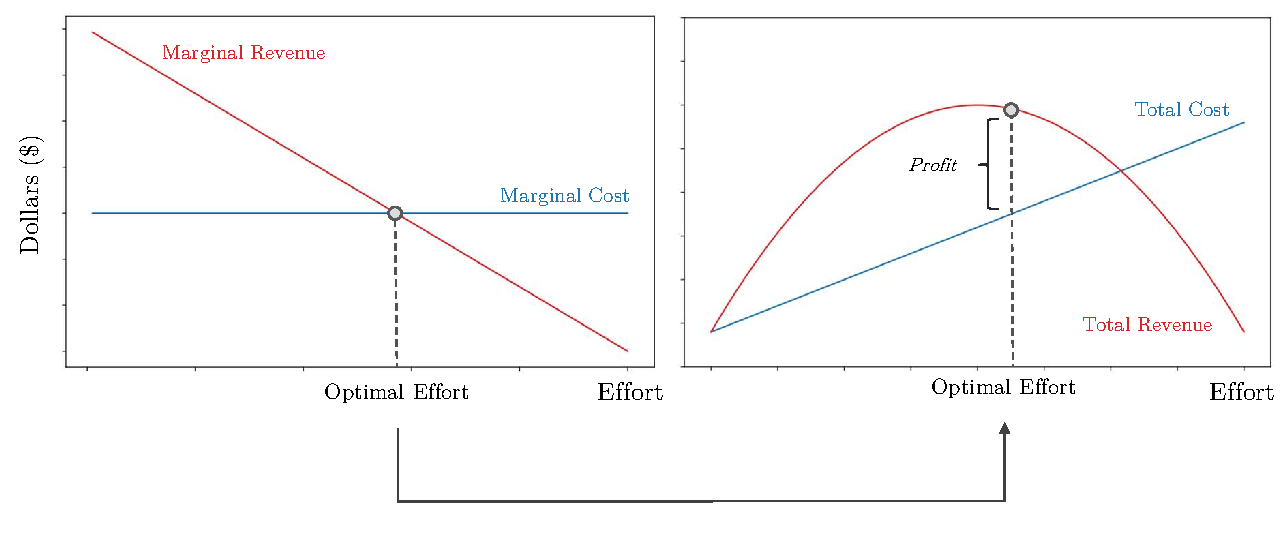
\includegraphics[scale=0.65]{figures/gordonschaefer.pdf}
    \captionsetup{width=0.9\textwidth}
    \caption{\textbf{Gordon-Schaefer model effort optimization for species harvesting.} Net Profit (\(\pi\)) can be obtained from the difference between Total Revenue and Total Cost.}
    \label{fig:gordonschafer}
\end{figure}

\subsubsection{Social Benefit}

To calculate the social welfare benefit of a foreign species on society, we can calculate the \textit{total social welfare} received by a population surrounding the foreign species and region in question. To determine the explicit dollar-value benefits of social welfare, we can utilize Sen's Welfare Function (which incorporates a Gini coefficient) to model the benefits of a particular species scaled to the region's income inequalities \cite{wikipediaSocialWelfare, worldbankWorldBank}. 

Therefore, we can express the \textit{total welfare benefit} (USD) \(W\) as a sum of individual benefits \(Y_i\), Gini coefficient \(G\), and regional population \(n\),

\begin{equation}
    W = (1 - G) \sum_{i=1}^n Y_i
\end{equation}

\subsubsection{Human Health Risk}

To calculate human health risk as an economic factor, we analyze the average detriment a species has to humans as a sum of individual risks based on the potential amount of money lost. The sum can again be scaled similarly to Sen's Welfare Function using the Gini coefficient. Data for the detrimental costs of a species to human society can be found for virtually any species, allowing us to assume generalizability \cite{fmrInvasiveSpecies}.

Therefore, we express the \textit{total human risk} (USD) \(R\) as a sum of individual risks \(R_i\), Gini coefficient \(G\), and regional population \(n\),

\begin{equation}
    R = (1 - G) \sum_{i=1}^n R_i 
\end{equation}

Therefore, we can express the total economic benefit of a given species in a region as the sum of economic profit (\(\pi\)) and social benefit (\(W\)) minus the human health risk (\(R\)).

\begin{equation}
    \text{Total Economic Benefit } = \pi + W - R
    \label{eq:economicimpact}
\end{equation}

So, we combine the Ecological (Equation~\ref{eq:ecologicalimpact}) and Economic (Equation~\ref{eq:economicimpact}) sub-scores as a coordinate pair to represent the trade-off between the two.

\begin{equation}
    \text{\textbf{Impact Score} } = (\text{Ecological Score, Economic Score}) = (100r + \chi, \hspace{0.05cm} \pi + W - R)
\end{equation}